\documentclass[UTF8,11pt]{ctexart}
\usepackage[a4paper,margin=22mm]{geometry}
\usepackage{amsmath,amssymb,bm,graphicx,adjustbox,fvextra,longtable,array}
\xeCJKDeclareCharClass{CJK}{"2160 -> "217F, "2460 -> "249B, "2200 -> "22FF}
\newcommand{\fitmath}[1]{\begin{adjustbox}{max width=\linewidth}$\displaystyle #1$\end{adjustbox}}
\setlength{\parindent}{0pt}\setlength{\parskip}{.65em}\renewcommand{\arraystretch}{1.3}
\sloppy\allowdisplaybreaks
\begin{document}
\section*{2020 年计算机统考 408 · 真题}
2020 年全国硕士研究生入学统一考试计算机学科专业基础综合试题


\subsection*{一、单项选择题（1～40 小题，每小题2 分，共80 分。下列每小题给出的四个选项中，只有一项符合题目要求）}

1. 将一个\(\displaystyle 10\times10\) 对称矩阵 \(\displaystyle M\) 的上三角部分的元素叫\(\displaystyle m_{i,\allowbreak j}\ (1\le i\le j\le10)\)按列优先存入C 语言的一维数组N 中，元素\(\displaystyle m_{7,\allowbreak 2}\)在N 中的下标是\_\_\_\_\_\_\_\_。


\begin{center}\begin{tabular}{>{\raggedright\arraybackslash}p{\dimexpr(\linewidth-8\tabcolsep)/4\relax}>{\raggedright\arraybackslash}p{\dimexpr(\linewidth-8\tabcolsep)/4\relax}>{\raggedright\arraybackslash}p{\dimexpr(\linewidth-8\tabcolsep)/4\relax}>{\raggedright\arraybackslash}p{\dimexpr(\linewidth-8\tabcolsep)/4\relax}}
\textbf{A.} 15 & \textbf{B.} 16 & \textbf{C.} 22 & \textbf{D.} 23\\[.35em]\end{tabular}\end{center}

2. 对空栈S 进行Push 和Pop 操作，入栈序列为 a, b, c, d, e，经过Push, Push, Pop, Push, Pop, Push, Push, Pop 操作后得到的出栈序列是\_\_\_\_\_\_\_\_。


\begin{center}\begin{tabular}{>{\raggedright\arraybackslash}p{\dimexpr(\linewidth-8\tabcolsep)/4\relax}>{\raggedright\arraybackslash}p{\dimexpr(\linewidth-8\tabcolsep)/4\relax}>{\raggedright\arraybackslash}p{\dimexpr(\linewidth-8\tabcolsep)/4\relax}>{\raggedright\arraybackslash}p{\dimexpr(\linewidth-8\tabcolsep)/4\relax}}
\textbf{A.} b, a, c & \textbf{B.} b, a, e & \textbf{C.} b, c, a & \textbf{D.} b, c, e\\[.35em]\end{tabular}\end{center}

3. 对于任意一棵高度为5 且有10 个结点的二叉树，若采用顺序存储结构保存，每个结点占1 个存储单元（仅存放结点的数据信息），则存放该二叉树需要的存储单元数量至少是\_\_\_\_\_\_\_\_。


\begin{center}\begin{tabular}{>{\raggedright\arraybackslash}p{\dimexpr(\linewidth-8\tabcolsep)/4\relax}>{\raggedright\arraybackslash}p{\dimexpr(\linewidth-8\tabcolsep)/4\relax}>{\raggedright\arraybackslash}p{\dimexpr(\linewidth-8\tabcolsep)/4\relax}>{\raggedright\arraybackslash}p{\dimexpr(\linewidth-8\tabcolsep)/4\relax}}
\textbf{A.} 31 & \textbf{B.} 16 & \textbf{C.} 15 & \textbf{D.} 10\\[.35em]\end{tabular}\end{center}

4. 已知森林F 及与之对应的二叉树T，若F 的先根遍历序列是a, b, c, d, e, f，中根遍历序列是b, a, d, f, e, c,则T 的后根遍历序列是\_\_\_\_\_\_\_\_。


\begin{center}\begin{tabular}{>{\raggedright\arraybackslash}p{\dimexpr(\linewidth-8\tabcolsep)/4\relax}>{\raggedright\arraybackslash}p{\dimexpr(\linewidth-8\tabcolsep)/4\relax}>{\raggedright\arraybackslash}p{\dimexpr(\linewidth-8\tabcolsep)/4\relax}>{\raggedright\arraybackslash}p{\dimexpr(\linewidth-8\tabcolsep)/4\relax}}
\textbf{A.} b, a, d, f, e, c & \textbf{B.} b, d, f, e, c, a & \textbf{C.} b, f, e, d, c, a & \textbf{D.} f, e, d, c, b, a\\[.35em]\end{tabular}\end{center}

5. 下列给定的关键字输入序列中，不能生成如下二叉排序树的是\_\_\_\_\_\_\_\_。


\begin{center}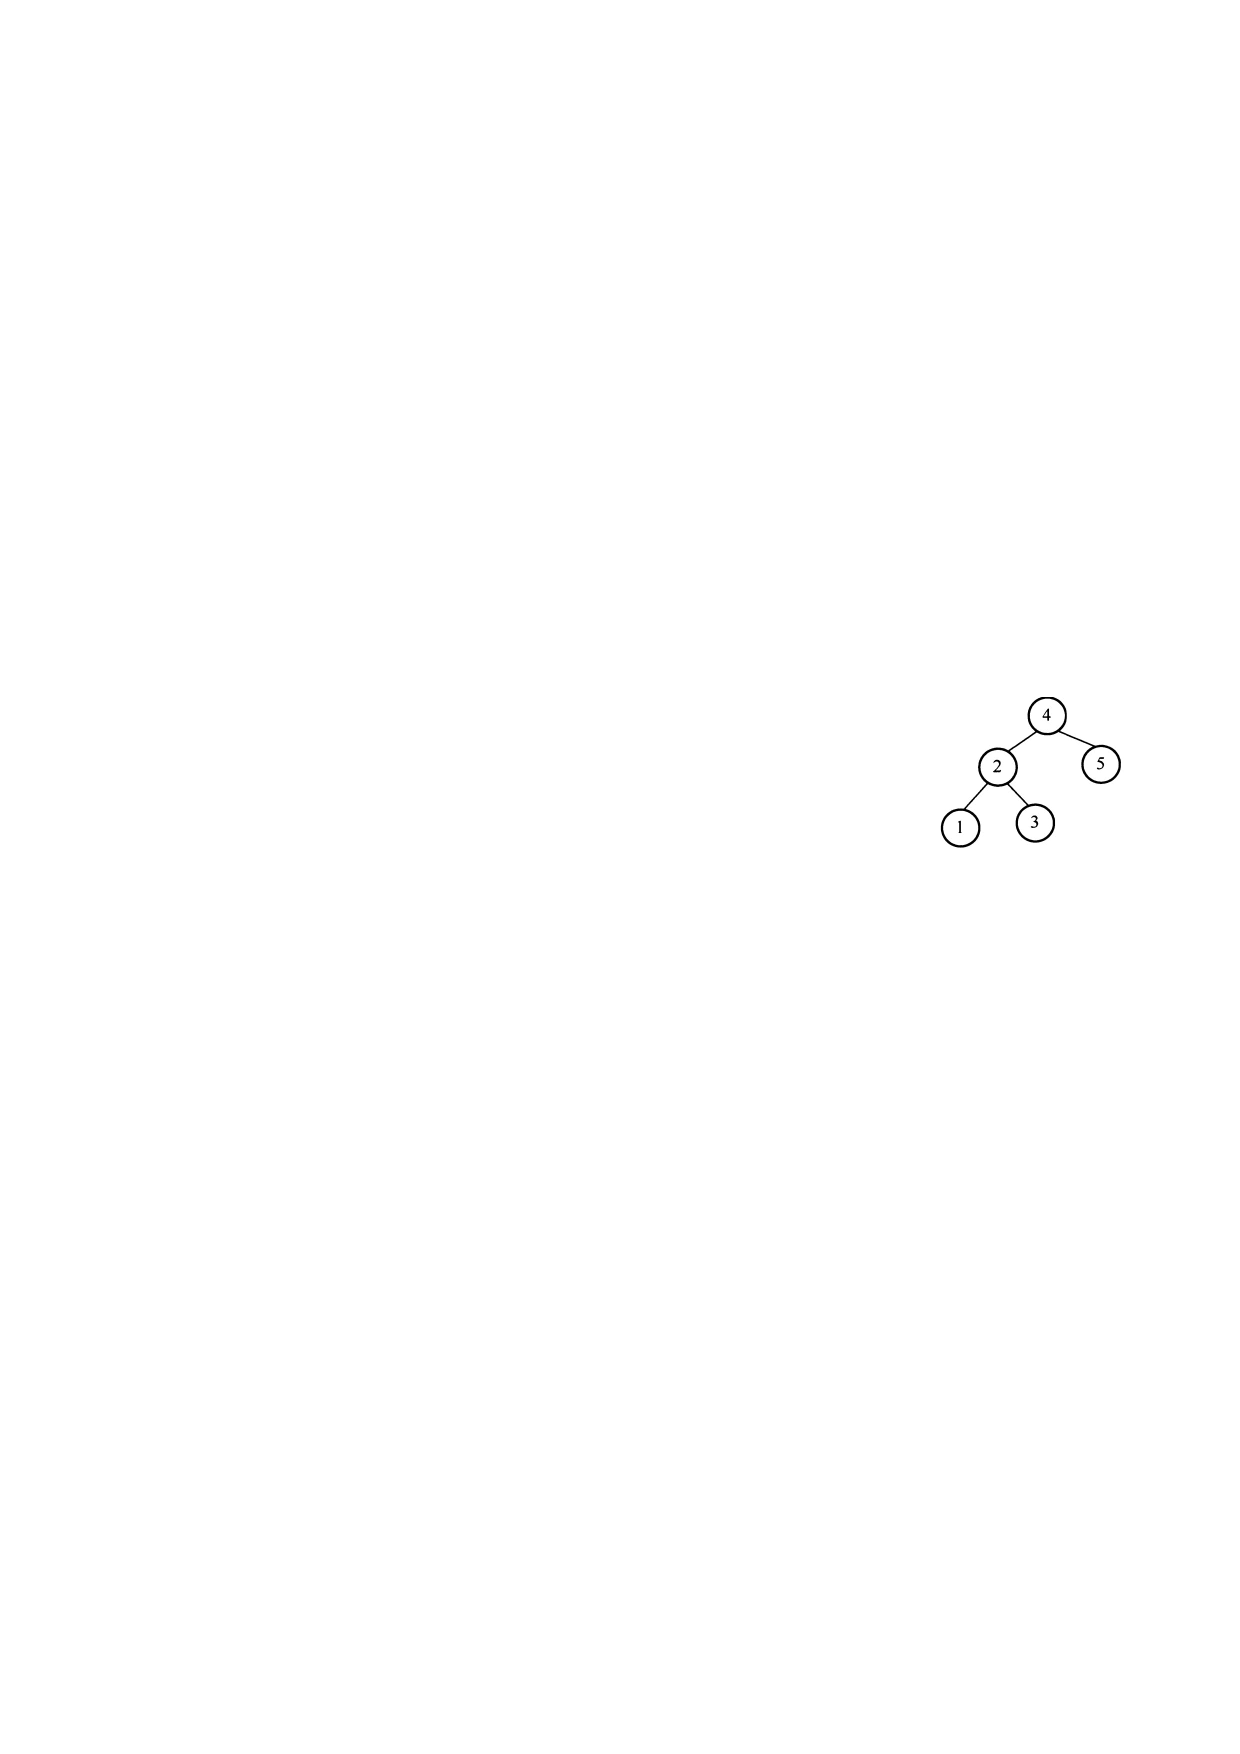
\includegraphics[width=.65\linewidth,height=.4\textheight,keepaspectratio]{../assets/figures/2020-questions-p001-b007.pdf}\end{center}

\begin{center}\begin{tabular}{>{\raggedright\arraybackslash}p{\dimexpr(\linewidth-8\tabcolsep)/4\relax}>{\raggedright\arraybackslash}p{\dimexpr(\linewidth-8\tabcolsep)/4\relax}>{\raggedright\arraybackslash}p{\dimexpr(\linewidth-8\tabcolsep)/4\relax}>{\raggedright\arraybackslash}p{\dimexpr(\linewidth-8\tabcolsep)/4\relax}}
\textbf{A.} 4, 5, 2, 1, 3 & \textbf{B.} 4, 5, 1, 2, 3 & \textbf{C.} 4, 2, 5, 3, 1 & \textbf{D.} 4, 2, 1, 3, 5\\[.35em]\end{tabular}\end{center}

6. 修改递归方式实现的图的深度优先搜索（DFS）算法，将输出（访问）顶点信息的语句移到退出递归前（即执行输出语句后立刻退出递归）。采用修改后的算法遍历有向无环图G，若输出结果中包含G 中的全部顶点，则输出的顶点序列是G 的\_\_\_\_\_\_\_\_。


\begin{center}\begin{tabular}{>{\raggedright\arraybackslash}p{\dimexpr(\linewidth-8\tabcolsep)/4\relax}>{\raggedright\arraybackslash}p{\dimexpr(\linewidth-8\tabcolsep)/4\relax}>{\raggedright\arraybackslash}p{\dimexpr(\linewidth-8\tabcolsep)/4\relax}>{\raggedright\arraybackslash}p{\dimexpr(\linewidth-8\tabcolsep)/4\relax}}
\textbf{A.} 拓扑有序序列 & \textbf{B.} 逆拓扑有序序列 & \textbf{C.} 广度优先搜索序列 & \textbf{D.} 深度优先搜索序列\\[.35em]\end{tabular}\end{center}

7. 已知无向图G 如下所示，使用克鲁斯卡尔（Kruskal）算法求图G 的最小生成树,加到最小生成树中的边依次是\_\_\_\_\_\_\_\_。


\begin{center}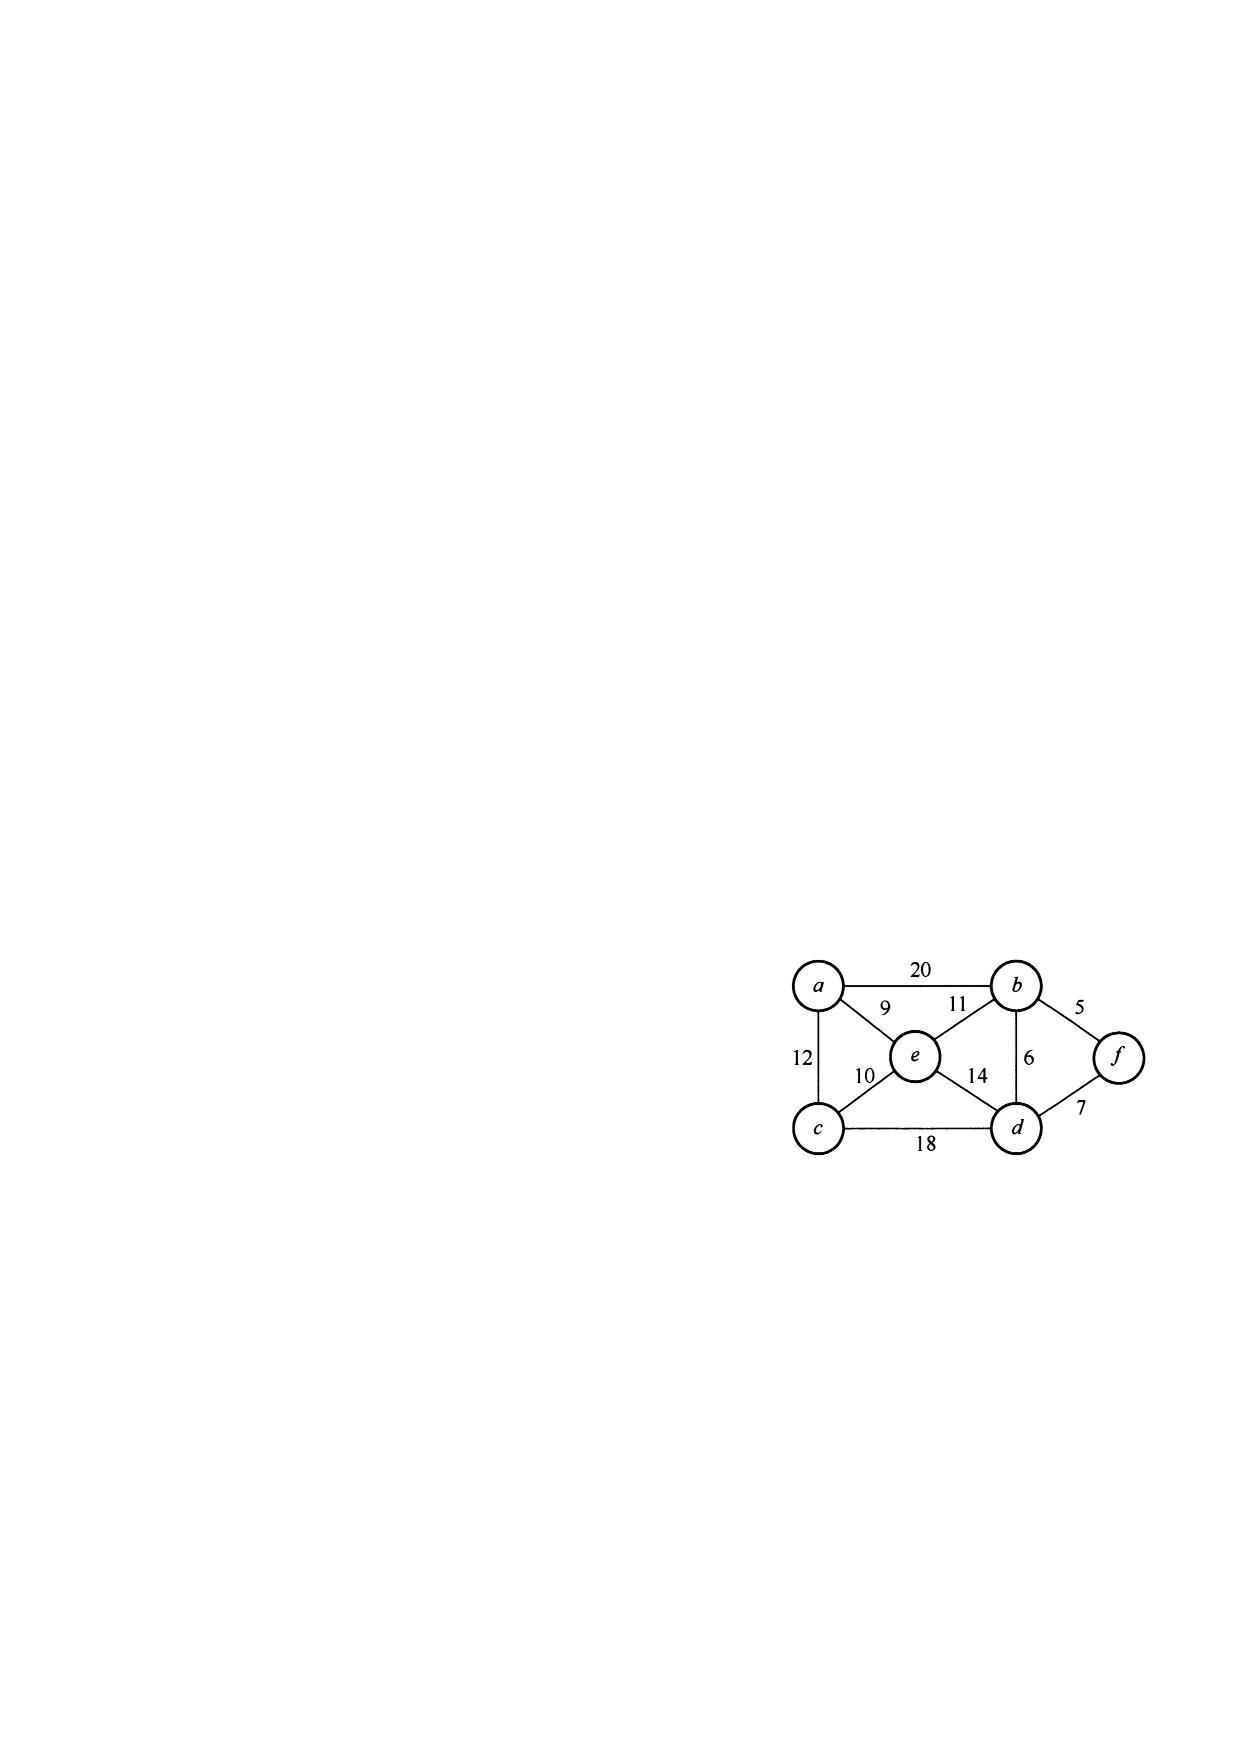
\includegraphics[width=.65\linewidth,height=.4\textheight,keepaspectratio]{../assets/figures/2020-questions-p001-b011.pdf}\end{center}

\begin{center}\begin{tabular}{>{\raggedright\arraybackslash}p{\dimexpr(\linewidth-4\tabcolsep)/2\relax}>{\raggedright\arraybackslash}p{\dimexpr(\linewidth-4\tabcolsep)/2\relax}}
\textbf{A.} (b, f), (b, d), (a, e), (c, e), (b, e) & \textbf{B.} (b, f), (b, d), (b, e), (a, e), (c, e)\\[.35em]
\textbf{C.} (a, e), (b, e), (c, e), (b, d), (b, f) & \textbf{D.} (a, e), (c, e), (b, e), (b, f), (b, d)\\[.35em]\end{tabular}\end{center}

8. 若使用AOE 网估算工程进度，则下列叙述中正确的是\_\_\_\_\_\_\_\_。


\begin{center}\begin{tabular}{>{\raggedright\arraybackslash}p{\dimexpr(\linewidth-4\tabcolsep)/2\relax}>{\raggedright\arraybackslash}p{\dimexpr(\linewidth-4\tabcolsep)/2\relax}}
\textbf{A.} 关键路径是从原点到汇点边数最多的一条路径 & \textbf{B.} 关键路径是从原点到汇点路径长度最长的路径\\[.35em]
\textbf{C.} 增加任一关键活动的时间不会延长工程的工期 & \textbf{D.} 缩短任一关键活动的时间将会缩短工程的工期\\[.35em]\end{tabular}\end{center}

9. 下列关于大根堆（至少含2 个元素）的叙述中，正确的是\_\_\_\_\_\_\_\_。 I. 可以将堆视为一棵完全二叉树 II. 可以采用顺序存储方式保存堆 III. 可以将堆视为一棵二叉排序树 IV. 堆中的次大值一定在根的下一层


\begin{center}\begin{tabular}{>{\raggedright\arraybackslash}p{\dimexpr(\linewidth-8\tabcolsep)/4\relax}>{\raggedright\arraybackslash}p{\dimexpr(\linewidth-8\tabcolsep)/4\relax}>{\raggedright\arraybackslash}p{\dimexpr(\linewidth-8\tabcolsep)/4\relax}>{\raggedright\arraybackslash}p{\dimexpr(\linewidth-8\tabcolsep)/4\relax}}
\textbf{A.} 仅I、II & \textbf{B.} 仅II、III & \textbf{C.} 仅I、II 和IV & \textbf{D.} 仅I、III 和IV\\[.35em]\end{tabular}\end{center}

10.依次将关键字5, 6, 9, 13, 8, 2, 12, 15 插入初始为空的4 阶B 树后，根结点中包含的关键字是\_\_\_\_\_\_\_\_。


\begin{center}\begin{tabular}{>{\raggedright\arraybackslash}p{\dimexpr(\linewidth-8\tabcolsep)/4\relax}>{\raggedright\arraybackslash}p{\dimexpr(\linewidth-8\tabcolsep)/4\relax}>{\raggedright\arraybackslash}p{\dimexpr(\linewidth-8\tabcolsep)/4\relax}>{\raggedright\arraybackslash}p{\dimexpr(\linewidth-8\tabcolsep)/4\relax}}
\textbf{A.} 8 & \textbf{B.} 6,9 & \textbf{C.} 8, 13 & \textbf{D.} 9, 12\\[.35em]\end{tabular}\end{center}

11.对大部分元素已有序的数组进行排序时，直接插入排序比简单选择排序效率更高，其原因是\_\_\_\_\_\_\_\_。 I. 直接插入排序过程中元素之间的比较次数更少 II. 直接插入排序过程中所需要的辅助空间更少 III. 直接插入排序过程中元素的移动次数更少


\begin{center}\begin{tabular}{>{\raggedright\arraybackslash}p{\dimexpr(\linewidth-8\tabcolsep)/4\relax}>{\raggedright\arraybackslash}p{\dimexpr(\linewidth-8\tabcolsep)/4\relax}>{\raggedright\arraybackslash}p{\dimexpr(\linewidth-8\tabcolsep)/4\relax}>{\raggedright\arraybackslash}p{\dimexpr(\linewidth-8\tabcolsep)/4\relax}}
\textbf{A.} 仅I & \textbf{B.} 仅III & \textbf{C.} 仅I、II & \textbf{D.} I、II 和III\\[.35em]\end{tabular}\end{center}

12.下列给出的部件中，其位数（宽度）一定与机器字长相同的是\_\_\_\_\_\_\_\_。 I. ALU II. 指令寄存器 III. 通用寄存器 IV. 浮点寄存器


\begin{center}\begin{tabular}{>{\raggedright\arraybackslash}p{\dimexpr(\linewidth-8\tabcolsep)/4\relax}>{\raggedright\arraybackslash}p{\dimexpr(\linewidth-8\tabcolsep)/4\relax}>{\raggedright\arraybackslash}p{\dimexpr(\linewidth-8\tabcolsep)/4\relax}>{\raggedright\arraybackslash}p{\dimexpr(\linewidth-8\tabcolsep)/4\relax}}
\textbf{A.} 仅 I、II & \textbf{B.} 仅 I、III & \textbf{C.} 仅 II、III & \textbf{D.} 仅II、III、IV\\[.35em]\end{tabular}\end{center}

13.已知带符号整数用补码表示，float 型数据用IEEE 754 标准表示，假定变量x 的类型只可能是int 或float,当x 的机器数为C800 0000H 时，x 的值可能是\_\_\_\_\_\_\_\_。


\begin{center}\begin{tabular}{>{\raggedright\arraybackslash}p{\dimexpr(\linewidth-8\tabcolsep)/4\relax}>{\raggedright\arraybackslash}p{\dimexpr(\linewidth-8\tabcolsep)/4\relax}>{\raggedright\arraybackslash}p{\dimexpr(\linewidth-8\tabcolsep)/4\relax}>{\raggedright\arraybackslash}p{\dimexpr(\linewidth-8\tabcolsep)/4\relax}}
\textbf{A.} \(\displaystyle -7\times2^{27}\) & \textbf{B.} \(\displaystyle -2^{16}\) & \textbf{C.} \(\displaystyle 2^{17}\) & \textbf{D.} \(\displaystyle 25\times2^{27}\)\\[.35em]\end{tabular}\end{center}

14.在按字节编址，采用小端方式的32 位计算机中，按边界对齐方式为以下C 语言结构型变量a 分配存储空间：


\begin{Verbatim}[breaklines,breakanywhere,fontsize=\small]
Struct record{
    short x1;
    int x2;
} a;
\end{Verbatim}

若a 的首地址为2020 FE00H，a 的成员变量x2 的机器数为1234 0000H，则其中34H 所在存储单元的地址是\_\_\_\_\_\_\_\_。


\begin{center}\begin{tabular}{>{\raggedright\arraybackslash}p{\dimexpr(\linewidth-8\tabcolsep)/4\relax}>{\raggedright\arraybackslash}p{\dimexpr(\linewidth-8\tabcolsep)/4\relax}>{\raggedright\arraybackslash}p{\dimexpr(\linewidth-8\tabcolsep)/4\relax}>{\raggedright\arraybackslash}p{\dimexpr(\linewidth-8\tabcolsep)/4\relax}}
\textbf{A.} 2020 FE03H & \textbf{B.} 2020 FE04H & \textbf{C.} 2020 FE05H & \textbf{D.} 2020 FE06H\\[.35em]\end{tabular}\end{center}

15.下列关于TLB 和Cache 的叙述中，错误的是\_\_\_\_\_\_\_\_。


\begin{center}\begin{tabular}{>{\raggedright\arraybackslash}p{\dimexpr(\linewidth-4\tabcolsep)/2\relax}>{\raggedright\arraybackslash}p{\dimexpr(\linewidth-4\tabcolsep)/2\relax}}
\textbf{A.} 命中率都与程序局部性有关 & \textbf{B.} 缺失后都需要去访问主存\\[.35em]
\textbf{C.} 缺失处理都可以由硬件实现 & \textbf{D.} 都由DRAM 存储器组成\\[.35em]\end{tabular}\end{center}

16.某计算机采用16 位定长指令字格式，操作码位数和寻址方式位数固定，指令系统有48 条指令， 支持直接、间接、立即、相对4 种寻址方式。单地址指令中，直接寻址方式的可寻址范围是\_\_\_\_\_\_\_\_。


\begin{center}\begin{tabular}{>{\raggedright\arraybackslash}p{\dimexpr(\linewidth-8\tabcolsep)/4\relax}>{\raggedright\arraybackslash}p{\dimexpr(\linewidth-8\tabcolsep)/4\relax}>{\raggedright\arraybackslash}p{\dimexpr(\linewidth-8\tabcolsep)/4\relax}>{\raggedright\arraybackslash}p{\dimexpr(\linewidth-8\tabcolsep)/4\relax}}
\textbf{A.} 0～255 & \textbf{B.} 0～1023 & \textbf{C.} －128～127 & \textbf{D.} －512～511\\[.35em]\end{tabular}\end{center}

17.下列给出的处理器类型中，理想情况下，CPI 为1 的是\_\_\_\_\_\_\_\_。 I. 单周期CPU II. 多周期CPU III. 基本流水线CPU IV. 超标量流水线CPU


\begin{center}\begin{tabular}{>{\raggedright\arraybackslash}p{\dimexpr(\linewidth-8\tabcolsep)/4\relax}>{\raggedright\arraybackslash}p{\dimexpr(\linewidth-8\tabcolsep)/4\relax}>{\raggedright\arraybackslash}p{\dimexpr(\linewidth-8\tabcolsep)/4\relax}>{\raggedright\arraybackslash}p{\dimexpr(\linewidth-8\tabcolsep)/4\relax}}
\textbf{A.} 仅I、II & \textbf{B.} 仅I、III & \textbf{C.} 仅II、IV & \textbf{D.} 仅III、IV\\[.35em]\end{tabular}\end{center}

18.下列关于“自陷”（Trap，也称陷阱）的叙述中，错误的是\_\_\_\_\_\_\_\_。


\begin{center}\begin{tabular}{>{\raggedright\arraybackslash}p{\dimexpr(\linewidth-4\tabcolsep)/2\relax}>{\raggedright\arraybackslash}p{\dimexpr(\linewidth-4\tabcolsep)/2\relax}}
\textbf{A.} 自陷是通过陷阱指令预先设定的一类外部中断事件 & \textbf{B.} 自陷可用于实现程序调试时的断点设置和单步跟踪\\[.35em]
\textbf{C.} 自陷发生后CPU 将转去执行操作系统内核相应程序 & \textbf{D.} 自陷处理完成后返回到陷阱指令的下一条指令执行\\[.35em]\end{tabular}\end{center}

19.QPI 总线是一种点对点全工同步串行总线，总线上的设备可同时接收和发送信息，每个方向可同时传输20 位信息（16 位数据+4 位校验位），每个QPI 数据包有80 位信息，分2 个时钟周期传送，每个时钟周期传递2 次。因此，QPI 总线带宽为：每秒传送次数×2B×2。若QPI 时钟频率为2.4GHz,则总线带宽为\_\_\_\_\_\_\_\_。


\begin{center}\begin{tabular}{>{\raggedright\arraybackslash}p{\dimexpr(\linewidth-8\tabcolsep)/4\relax}>{\raggedright\arraybackslash}p{\dimexpr(\linewidth-8\tabcolsep)/4\relax}>{\raggedright\arraybackslash}p{\dimexpr(\linewidth-8\tabcolsep)/4\relax}>{\raggedright\arraybackslash}p{\dimexpr(\linewidth-8\tabcolsep)/4\relax}}
\textbf{A.} 4.\allowbreak{}8GBps & \textbf{B.} 9.\allowbreak{}6GBps & \textbf{C.} 19.\allowbreak{}2GBps & \textbf{D.} 38.\allowbreak{}4GBps\\[.35em]\end{tabular}\end{center}

20.下列事件中，属于外部中断事件的是\_\_\_\_\_\_\_\_。 I. 访存时缺页 II. 定时器到时 III. 网络数据包到达


\begin{center}\begin{tabular}{>{\raggedright\arraybackslash}p{\dimexpr(\linewidth-8\tabcolsep)/4\relax}>{\raggedright\arraybackslash}p{\dimexpr(\linewidth-8\tabcolsep)/4\relax}>{\raggedright\arraybackslash}p{\dimexpr(\linewidth-8\tabcolsep)/4\relax}>{\raggedright\arraybackslash}p{\dimexpr(\linewidth-8\tabcolsep)/4\relax}}
\textbf{A.} 仅 I、II & \textbf{B.} 仅 I、III & \textbf{C.} 仅II、III & \textbf{D.} I、II 和III\\[.35em]\end{tabular}\end{center}

21.外部中断包括不可屏蔽中断（NMI）和可屏蔽中断，下列关于外部中断的叙述中，错误的是\_\_\_\_\_\_\_\_。


\begin{center}\begin{tabular}{>{\raggedright\arraybackslash}p{\dimexpr(\linewidth-4\tabcolsep)/2\relax}>{\raggedright\arraybackslash}p{\dimexpr(\linewidth-4\tabcolsep)/2\relax}}
\textbf{A.} CPU 处于关中断状态时，也能响应NMI 请求 & \\[.35em]\end{tabular}\end{center}

\begin{center}\begin{tabular}{>{\raggedright\arraybackslash}p{\dimexpr(\linewidth-4\tabcolsep)/2\relax}>{\raggedright\arraybackslash}p{\dimexpr(\linewidth-4\tabcolsep)/2\relax}}
\textbf{B.} 一旦可屏蔽中断请求信号有效，CPU 将立即响应 & \textbf{C.} 不可屏蔽中断的优先级比可屏蔽中断的优先级高\\[.35em]
\textbf{D.} 可通过中断屏蔽字改变可屏蔽中断的处理优先级 & \\[.35em]\end{tabular}\end{center}

22.若设备采用周期挪用DMA 方式进行输入和输出，每次DMA 传送的数据块大小为512 字节，相应的I/O 接口中有一个32 位数数据缓冲寄存器。对于数据输入过程，下列叙述中，错误的是\_\_\_\_\_\_\_\_。


\begin{center}\begin{tabular}{>{\raggedright\arraybackslash}p{\dimexpr(\linewidth-4\tabcolsep)/2\relax}>{\raggedright\arraybackslash}p{\dimexpr(\linewidth-4\tabcolsep)/2\relax}}
\textbf{A.} 每准备好32 位数据，DMA 控制器就发出一次总线请求 & \textbf{B.} 相对于CPU，DMA 控制器的总线使用权的优先级更高\\[.35em]
\textbf{C.} 在整个数据块的传送过程中，CPU 不可以访问主存储器 & \textbf{D.} 数据块传送结束时，会产生“DMA 传送结束”中断请求\\[.35em]\end{tabular}\end{center}

23.若多个进程共享同一个文件F，则下列叙述中，正确的是\_\_\_\_\_\_\_\_。


\begin{center}\begin{tabular}{>{\raggedright\arraybackslash}p{\dimexpr(\linewidth-4\tabcolsep)/2\relax}>{\raggedright\arraybackslash}p{\dimexpr(\linewidth-4\tabcolsep)/2\relax}}
\textbf{A.} 各进程只能用“读”方式打开文件F & \textbf{B.} 在系统打开文件表中仅有一个表项包含F 的属性\\[.35em]
\textbf{C.} 各进程的用户打开文件表中关于F 的表项内容相同 & \textbf{D.} 进程关闭F 时，系统删除F 在系统打开文件表中的表项\\[.35em]\end{tabular}\end{center}

24.下列选项中，支持文件长度可变、随机访问的磁盘存储空间分配方式是\_\_\_\_\_\_\_\_。


\begin{center}\begin{tabular}{>{\raggedright\arraybackslash}p{\dimexpr(\linewidth-8\tabcolsep)/4\relax}>{\raggedright\arraybackslash}p{\dimexpr(\linewidth-8\tabcolsep)/4\relax}>{\raggedright\arraybackslash}p{\dimexpr(\linewidth-8\tabcolsep)/4\relax}>{\raggedright\arraybackslash}p{\dimexpr(\linewidth-8\tabcolsep)/4\relax}}
\textbf{A.} 索引分配 & \textbf{B.} 链接分配 & \textbf{C.} 连续分配 & \textbf{D.} 动态分区分配\\[.35em]\end{tabular}\end{center}

25.下列与中断相关的操作中，由操作系统完成的是\_\_\_\_\_\_\_\_。 I. 保存被中断程序的中断点 II. 提供中断服务 III. 初始化中断向量表 IV. 保存中断屏蔽字


\begin{center}\begin{tabular}{>{\raggedright\arraybackslash}p{\dimexpr(\linewidth-8\tabcolsep)/4\relax}>{\raggedright\arraybackslash}p{\dimexpr(\linewidth-8\tabcolsep)/4\relax}>{\raggedright\arraybackslash}p{\dimexpr(\linewidth-8\tabcolsep)/4\relax}>{\raggedright\arraybackslash}p{\dimexpr(\linewidth-8\tabcolsep)/4\relax}}
\textbf{A.} 仅I、II & \textbf{B.} 仅I、II、IV & \textbf{C.} 仅III、IV & \textbf{D.} 仅II、III、IV\\[.35em]\end{tabular}\end{center}

26.下列与进程调度有关的因素中，在设计多级反馈队列调度算法时需要考虑的是\_\_\_\_\_\_\_\_。 I. 就绪队列的数量 II. 就绪队列的优先级 III. 各就绪队列的调度算法 IV. 进程在就绪队列间的迁移条件


\begin{center}\begin{tabular}{>{\raggedright\arraybackslash}p{\dimexpr(\linewidth-8\tabcolsep)/4\relax}>{\raggedright\arraybackslash}p{\dimexpr(\linewidth-8\tabcolsep)/4\relax}>{\raggedright\arraybackslash}p{\dimexpr(\linewidth-8\tabcolsep)/4\relax}>{\raggedright\arraybackslash}p{\dimexpr(\linewidth-8\tabcolsep)/4\relax}}
\textbf{A.} 仅I、II & \textbf{B.} 仅III、IV & \textbf{C.} 仅II 、III、IV & \textbf{D.} I、II、III 和IV\\[.35em]\end{tabular}\end{center}

27.某系统中有A、B 两类资源各6 个，t 时刻资源分配及需求情况如下表所示


\begin{center}\begin{adjustbox}{max width=\linewidth}\begin{tabular}{|>{\raggedright\arraybackslash}p{\dimexpr(\linewidth-10\tabcolsep-6\arrayrulewidth)/5\relax}|>{\raggedright\arraybackslash}p{\dimexpr(\linewidth-10\tabcolsep-6\arrayrulewidth)/5\relax}|>{\raggedright\arraybackslash}p{\dimexpr(\linewidth-10\tabcolsep-6\arrayrulewidth)/5\relax}|>{\raggedright\arraybackslash}p{\dimexpr(\linewidth-10\tabcolsep-6\arrayrulewidth)/5\relax}|>{\raggedright\arraybackslash}p{\dimexpr(\linewidth-10\tabcolsep-6\arrayrulewidth)/5\relax}|}\hline
进程 & A已分配数量 & B已分配数量 & A需求总量 & B需求总量\\\hline
P1 & 2 & 3 & 4 & 4\\\hline
P2 & 2 & 1 & 3 & 1\\\hline
P3 & 1 & 2 & 3 & 4\\\hline\end{tabular}\end{adjustbox}\end{center}

t 时刻安全性检测的结果是\_\_\_\_\_\_\_\_。


\begin{center}\begin{tabular}{>{\raggedright\arraybackslash}p{\dimexpr(\linewidth-4\tabcolsep)/2\relax}>{\raggedright\arraybackslash}p{\dimexpr(\linewidth-4\tabcolsep)/2\relax}}
\textbf{A.} 存在安全序列P1、P2、P3 & \textbf{B.} 存在安全序列P2、P1、P3\\[.35em]
\textbf{C.} 存在安全序列P2、P3、P1 & \textbf{D.} 不存在安全序列\\[.35em]\end{tabular}\end{center}

28.下列因素中，影响请求分页系统有效（平均）访存时间的是\_\_\_\_\_\_\_\_。 I. 缺页率 II. 磁盘读写时间 III. 内存访问时间 IV. 执行缺页处理程序的CPU 时间


\begin{center}\begin{tabular}{>{\raggedright\arraybackslash}p{\dimexpr(\linewidth-8\tabcolsep)/4\relax}>{\raggedright\arraybackslash}p{\dimexpr(\linewidth-8\tabcolsep)/4\relax}>{\raggedright\arraybackslash}p{\dimexpr(\linewidth-8\tabcolsep)/4\relax}>{\raggedright\arraybackslash}p{\dimexpr(\linewidth-8\tabcolsep)/4\relax}}
\textbf{A.} 仅II、III & \textbf{B.} 仅I、IV & \textbf{C.} 仅I、III、IV & \textbf{D.} I、II、III 和IV\\[.35em]\end{tabular}\end{center}

29.下列关于父进程与子进程的叙述中，错误的是\_\_\_\_\_\_\_\_。


\begin{center}\begin{tabular}{>{\raggedright\arraybackslash}p{\dimexpr(\linewidth-4\tabcolsep)/2\relax}>{\raggedright\arraybackslash}p{\dimexpr(\linewidth-4\tabcolsep)/2\relax}}
\textbf{A.} 父进程与子进程可以并发执行 & \textbf{B.} 父进程与子进程共享虚拟地址空间\\[.35em]
\textbf{C.} 父进程与子进程有不同的进程控制块 & \textbf{D.} 父进程与子进程不能同时使用同一临界资源\\[.35em]\end{tabular}\end{center}

30.对于具备设备独立性的系统，下列叙述中，错误的是\_\_\_\_\_\_\_\_。


\begin{center}\begin{tabular}{>{\raggedright\arraybackslash}p{\dimexpr(\linewidth-4\tabcolsep)/2\relax}>{\raggedright\arraybackslash}p{\dimexpr(\linewidth-4\tabcolsep)/2\relax}}
\textbf{A.} 可以使用文件名访问物理设备 & \textbf{B.} 用户程序使用逻辑设备名访问物理设备\\[.35em]
\textbf{C.} 需要建立逻辑设备与物理设备之间的映射关系 & \textbf{D.} 更换物理设备后必须修改访问该设备的应用程序\\[.35em]\end{tabular}\end{center}

31.某文件系统的目录项由文件名和索引结点号构成。若每个目录项长度为64 字节，其中4 字节存放索引结点号，60 字节存放文件名。文件名由小写英文字母构成，则该文件系统能创建的文件数量的上限为\_\_\_\_\_\_\_\_。


\begin{center}\begin{tabular}{>{\raggedright\arraybackslash}p{\dimexpr(\linewidth-8\tabcolsep)/4\relax}>{\raggedright\arraybackslash}p{\dimexpr(\linewidth-8\tabcolsep)/4\relax}>{\raggedright\arraybackslash}p{\dimexpr(\linewidth-8\tabcolsep)/4\relax}>{\raggedright\arraybackslash}p{\dimexpr(\linewidth-8\tabcolsep)/4\relax}}
\textbf{A.} \(\displaystyle 2^{26}\) & \textbf{B.} \(\displaystyle 2^{32}\) & \textbf{C.} \(\displaystyle 2^{60}\) & \textbf{D.} \(\displaystyle 2^{64}\)\\[.35em]\end{tabular}\end{center}

32.下列准则中，实现临界区互斥机制必须遵循的是\_\_\_\_\_\_\_\_。 I. 两个进程不能同时进入临界区 II. 允许进程访问空闲的临界资源 III. 进程等待进入临界区的时间是有限的 IV. 不能进入临界区的执行态进程立即放弃CPU


\begin{center}\begin{tabular}{>{\raggedright\arraybackslash}p{\dimexpr(\linewidth-8\tabcolsep)/4\relax}>{\raggedright\arraybackslash}p{\dimexpr(\linewidth-8\tabcolsep)/4\relax}>{\raggedright\arraybackslash}p{\dimexpr(\linewidth-8\tabcolsep)/4\relax}>{\raggedright\arraybackslash}p{\dimexpr(\linewidth-8\tabcolsep)/4\relax}}
\textbf{A.} 仅 I、IV & \textbf{B.} 仅 II、III & \textbf{C.} 仅 I、II、III & \textbf{D.} 仅 I、III、IV\\[.35em]\end{tabular}\end{center}

33.下图描述的协议要素是\_\_\_\_\_\_\_\_。


\begin{center}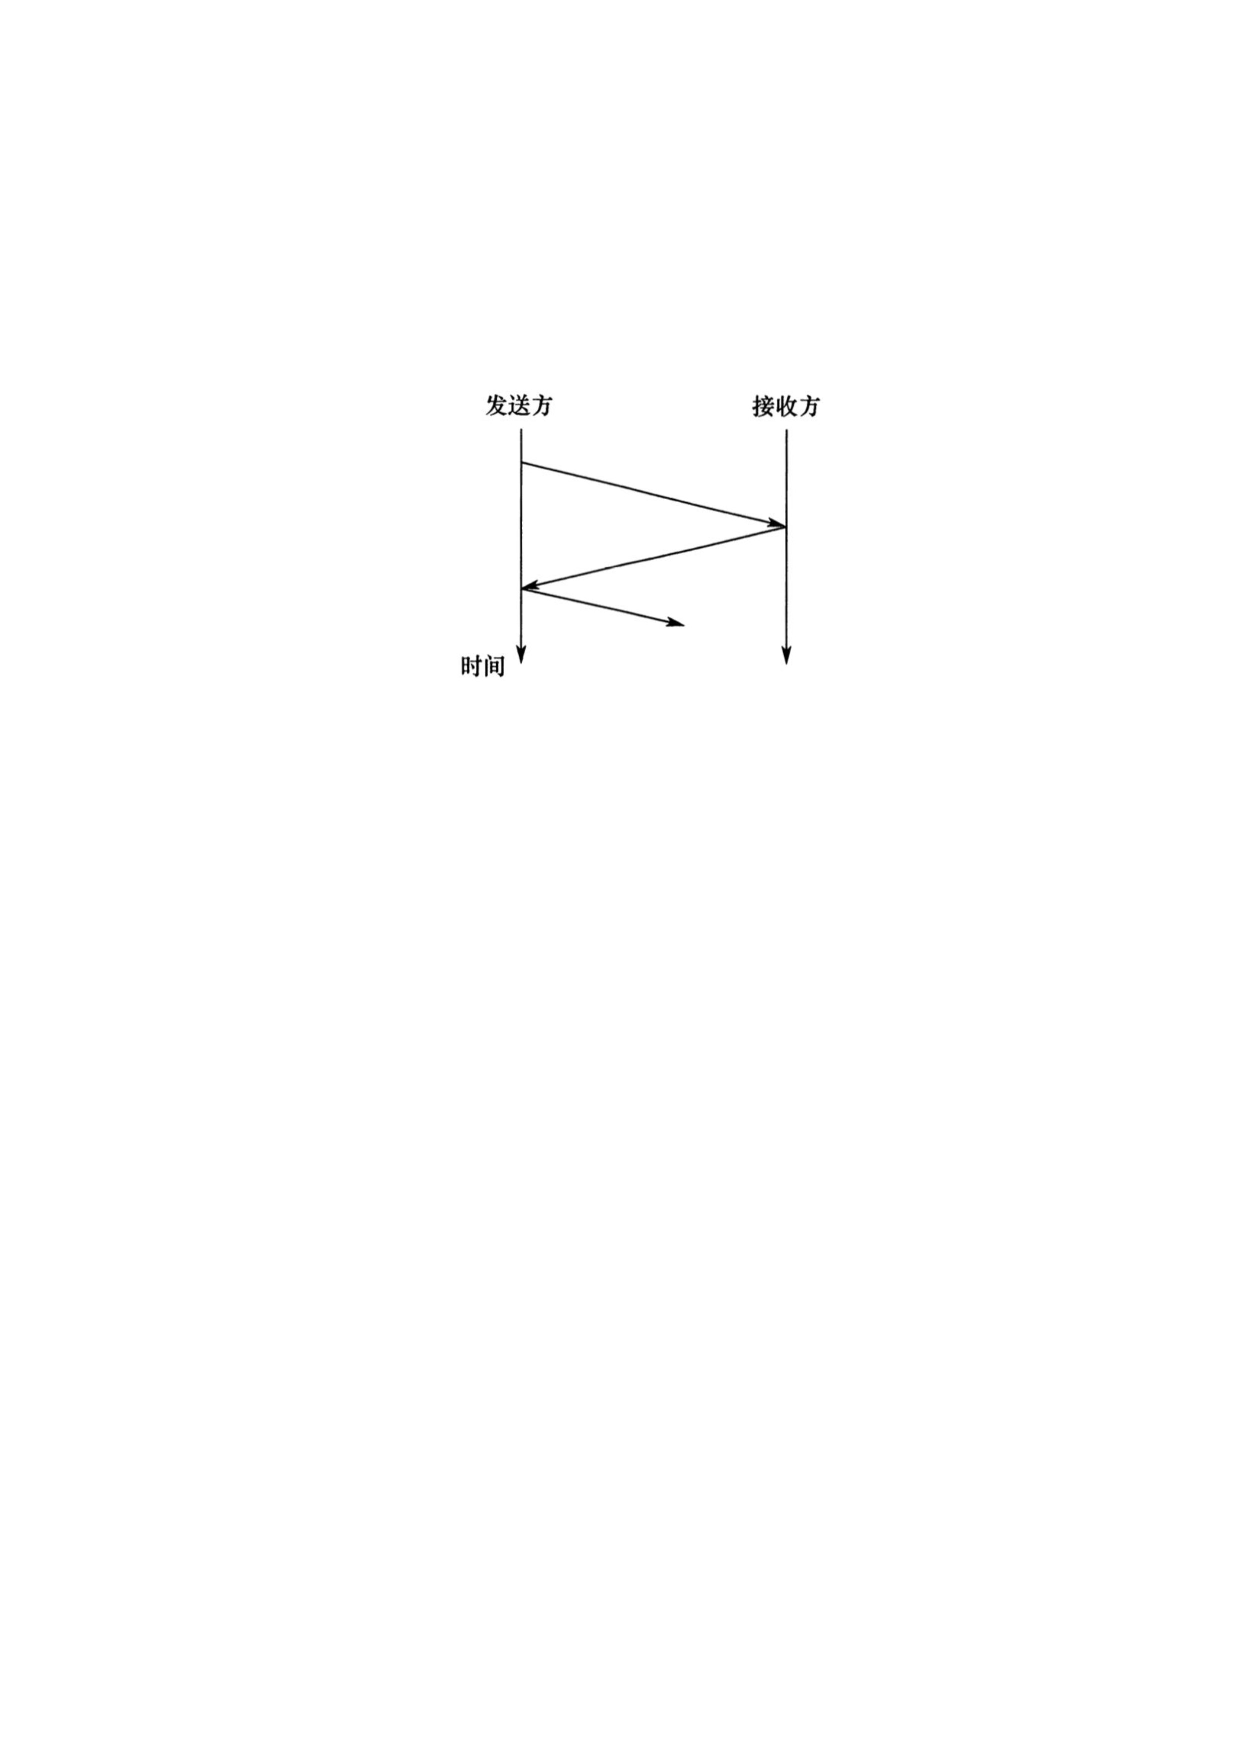
\includegraphics[width=.65\linewidth,height=.4\textheight,keepaspectratio]{../assets/figures/2020-questions-p004-b003.pdf}\end{center}

I. 语法 II. 语义 III. 时序


\begin{center}\begin{tabular}{>{\raggedright\arraybackslash}p{\dimexpr(\linewidth-8\tabcolsep)/4\relax}>{\raggedright\arraybackslash}p{\dimexpr(\linewidth-8\tabcolsep)/4\relax}>{\raggedright\arraybackslash}p{\dimexpr(\linewidth-8\tabcolsep)/4\relax}>{\raggedright\arraybackslash}p{\dimexpr(\linewidth-8\tabcolsep)/4\relax}}
\textbf{A.} 仅I & \textbf{B.} 仅II & \textbf{C.} 仅III & \textbf{D.} I、II 和III\\[.35em]\end{tabular}\end{center}

34.下列关于虚电路网络的叙述中，错误的是\_\_\_\_\_\_\_\_。


\begin{center}\begin{tabular}{>{\raggedright\arraybackslash}p{\dimexpr(\linewidth-4\tabcolsep)/2\relax}>{\raggedright\arraybackslash}p{\dimexpr(\linewidth-4\tabcolsep)/2\relax}}
\textbf{A.} 可以确保数据分组传输顺序 & \textbf{B.} 需要为每条虚电路预分配带宽\\[.35em]
\textbf{C.} 建立虚电路时需要进行路由选择 & \textbf{D.} 依据虚电路号（VCID）进行数据分组转发\\[.35em]\end{tabular}\end{center}

35.在下图所示的网络中，冲突域和广播域的个数分别是\_\_\_\_\_\_\_\_。


\begin{center}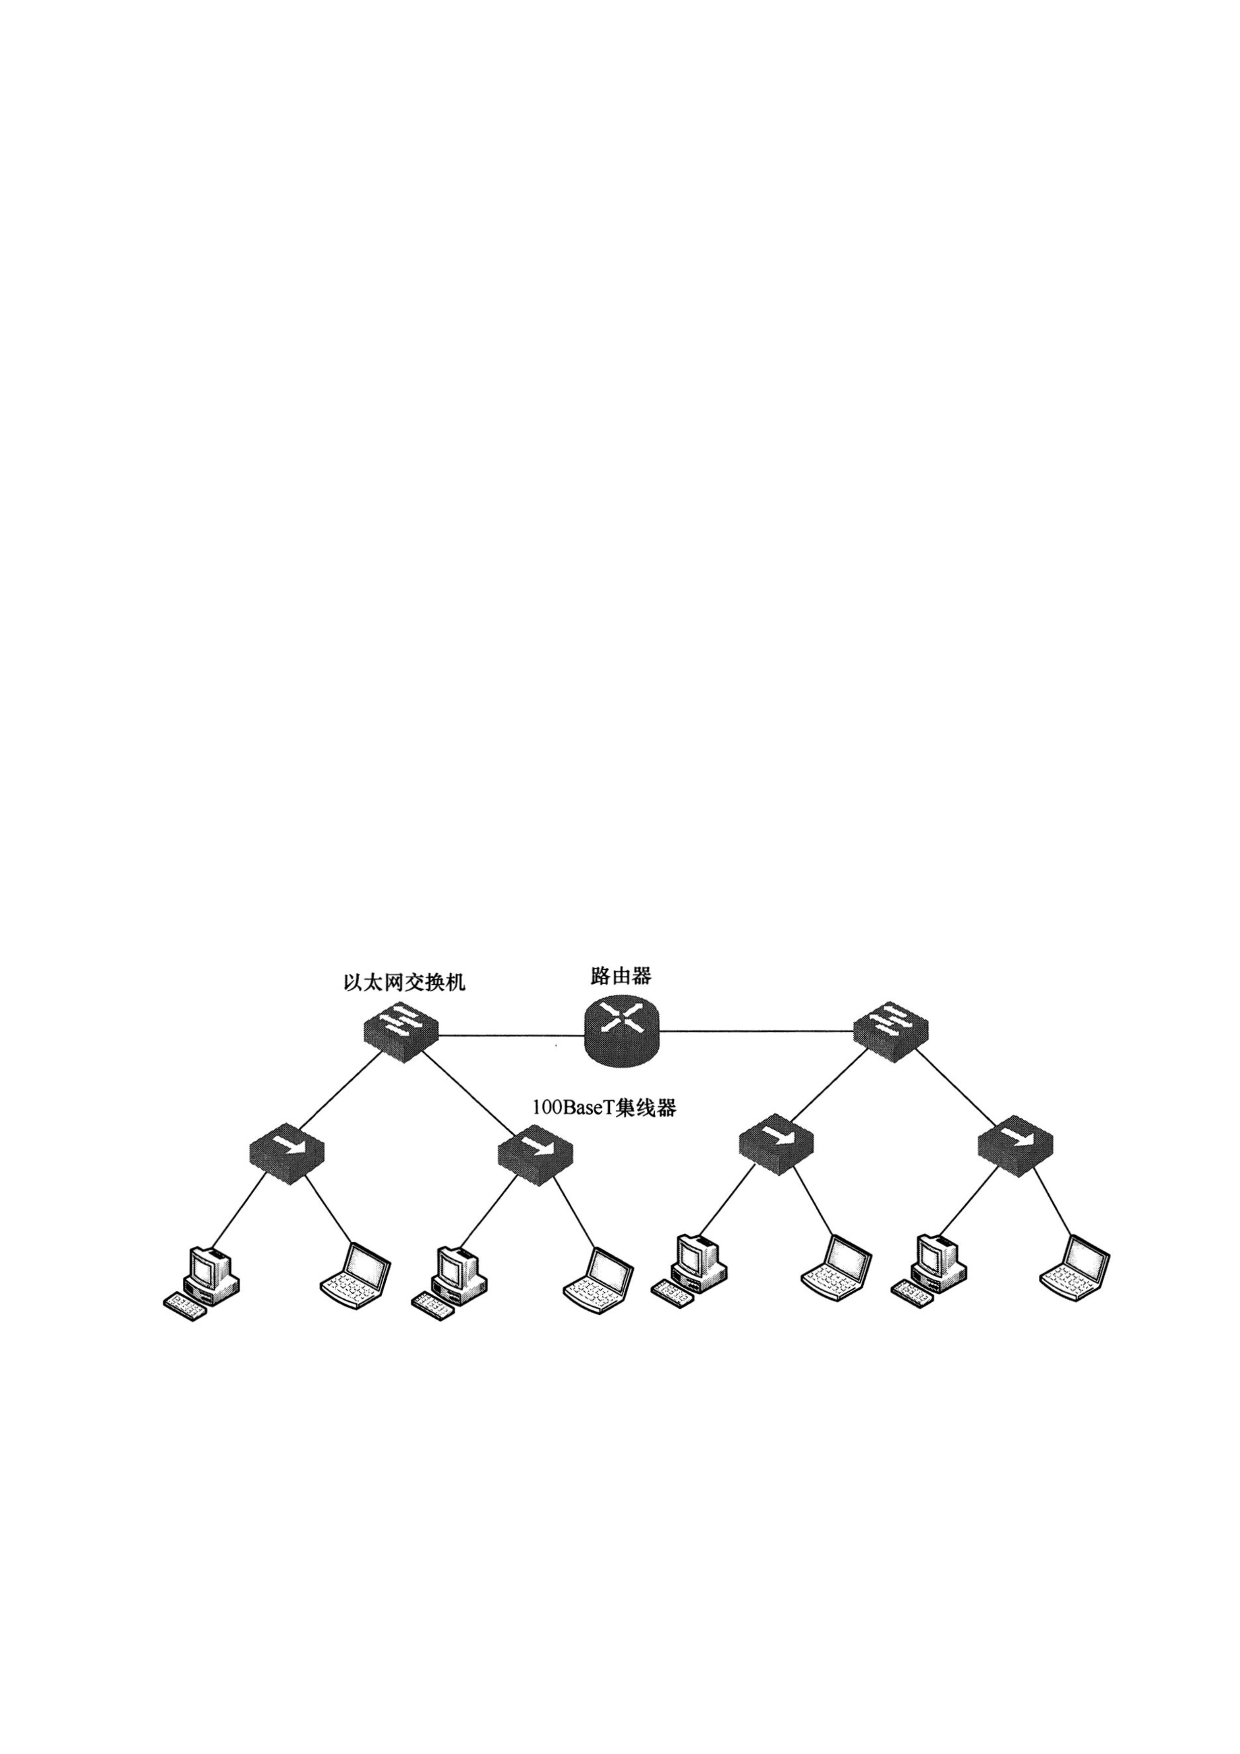
\includegraphics[width=.65\linewidth,height=.4\textheight,keepaspectratio]{../assets/figures/2020-questions-p004-b007.pdf}\end{center}

\begin{center}\begin{tabular}{>{\raggedright\arraybackslash}p{\dimexpr(\linewidth-8\tabcolsep)/4\relax}>{\raggedright\arraybackslash}p{\dimexpr(\linewidth-8\tabcolsep)/4\relax}>{\raggedright\arraybackslash}p{\dimexpr(\linewidth-8\tabcolsep)/4\relax}>{\raggedright\arraybackslash}p{\dimexpr(\linewidth-8\tabcolsep)/4\relax}}
\textbf{A.} 2, 2 & \textbf{B.} 2, 4 & \textbf{C.} 4, 2 & \textbf{D.} 4, 4\\[.35em]\end{tabular}\end{center}

36.假设主机甲采用停–等协议向主机乙发送数据帧，数据帧长与确认帧长均为1000B，数据传输速率是10kbps，单向传播延时是200ms。则甲的最大信道利用率为\_\_\_\_\_\_\_\_。


\begin{center}\begin{tabular}{>{\raggedright\arraybackslash}p{\dimexpr(\linewidth-8\tabcolsep)/4\relax}>{\raggedright\arraybackslash}p{\dimexpr(\linewidth-8\tabcolsep)/4\relax}>{\raggedright\arraybackslash}p{\dimexpr(\linewidth-8\tabcolsep)/4\relax}>{\raggedright\arraybackslash}p{\dimexpr(\linewidth-8\tabcolsep)/4\relax}}
\textbf{A.} 80\% & \textbf{B.} 66.\allowbreak{}7\% & \textbf{C.} 44.\allowbreak{}4\% & \textbf{D.} 40\%\\[.35em]\end{tabular}\end{center}

37.某IEEE 802.11 无线局域网中，主机H 与AP 之间发送或接收CSMA/CA 帧的过程如下图所示。 在H 或AP 发送帧前所等待的帧间间隔时间（IFS）中，最长的是\_\_\_\_\_\_\_\_。


\begin{center}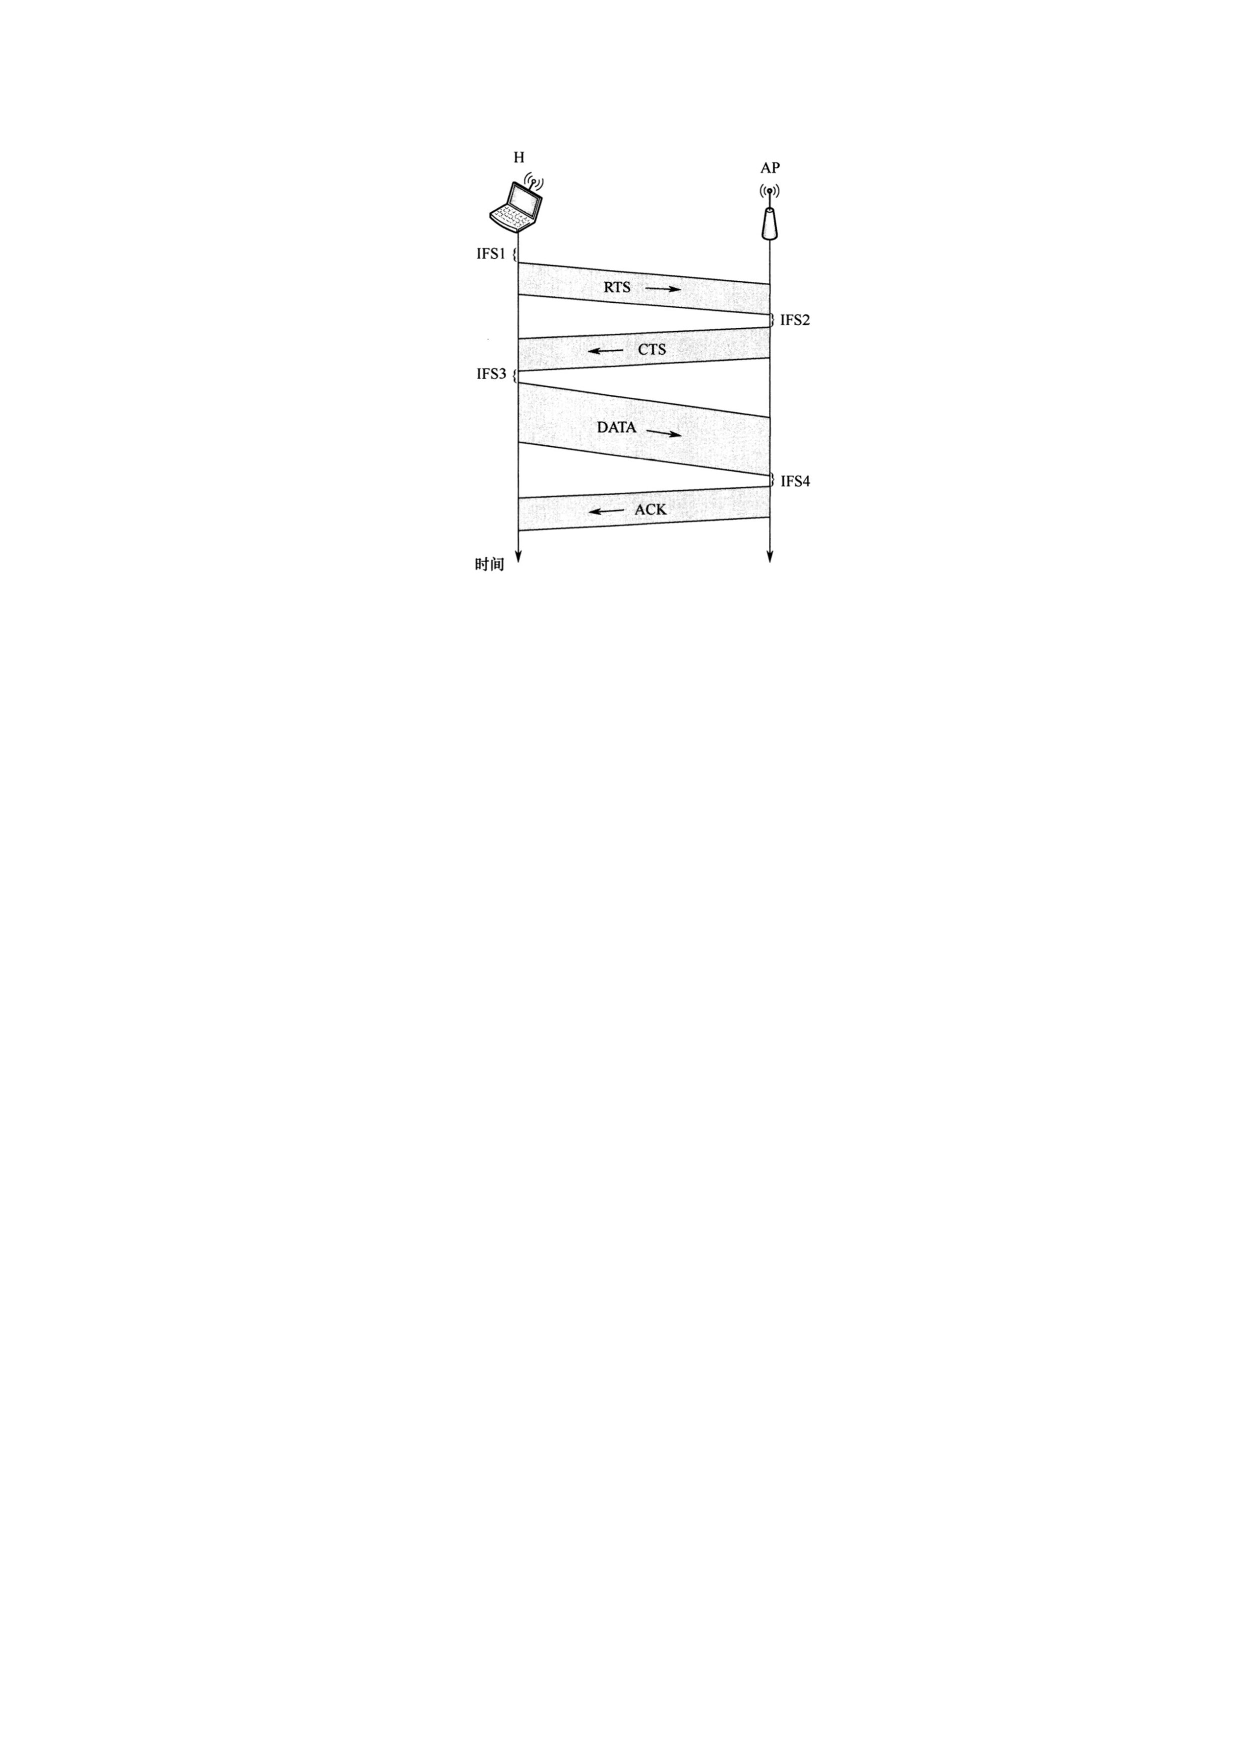
\includegraphics[width=.65\linewidth,height=.4\textheight,keepaspectratio]{../assets/figures/2020-questions-p005-b001.pdf}\end{center}

\begin{center}\begin{tabular}{>{\raggedright\arraybackslash}p{\dimexpr(\linewidth-8\tabcolsep)/4\relax}>{\raggedright\arraybackslash}p{\dimexpr(\linewidth-8\tabcolsep)/4\relax}>{\raggedright\arraybackslash}p{\dimexpr(\linewidth-8\tabcolsep)/4\relax}>{\raggedright\arraybackslash}p{\dimexpr(\linewidth-8\tabcolsep)/4\relax}}
\textbf{A.} IFS1 & \textbf{B.} IFS2 & \textbf{C.} IFS3 & \textbf{D.} IFS4\\[.35em]\end{tabular}\end{center}

38.若主机甲与主机乙已建立一条TCP 连接，最大段长（MSS）为1KB，往返时间（RTT）为 2ms，则在不出现拥塞的前提下，拥塞窗口从8KB 增长到32KB 所需的最长时间是\_\_\_\_\_\_\_\_。


\begin{center}\begin{tabular}{>{\raggedright\arraybackslash}p{\dimexpr(\linewidth-8\tabcolsep)/4\relax}>{\raggedright\arraybackslash}p{\dimexpr(\linewidth-8\tabcolsep)/4\relax}>{\raggedright\arraybackslash}p{\dimexpr(\linewidth-8\tabcolsep)/4\relax}>{\raggedright\arraybackslash}p{\dimexpr(\linewidth-8\tabcolsep)/4\relax}}
\textbf{A.} 4ms & \textbf{B.} 8ms & \textbf{C.} 24ms & \textbf{D.} 48ms\\[.35em]\end{tabular}\end{center}

39.若主机甲与主机乙建立TCP 连接时，发送的SYN 段中的序号为1000，在断开连接时，甲发送给乙的FIN 段中的序号为5001，则在无任何重传的情况下，甲向乙已经发送的应用层数据的字节数为\_\_\_\_\_\_\_\_。


\begin{center}\begin{tabular}{>{\raggedright\arraybackslash}p{\dimexpr(\linewidth-8\tabcolsep)/4\relax}>{\raggedright\arraybackslash}p{\dimexpr(\linewidth-8\tabcolsep)/4\relax}>{\raggedright\arraybackslash}p{\dimexpr(\linewidth-8\tabcolsep)/4\relax}>{\raggedright\arraybackslash}p{\dimexpr(\linewidth-8\tabcolsep)/4\relax}}
\textbf{A.} 4002 & \textbf{B.} 4001 & \textbf{C.} 4000 & \textbf{D.} 3999\\[.35em]\end{tabular}\end{center}

40.假设下图所示网络中的本地域名服务器只提供递归查询服务，其他域名服务器均只提供迭代查询服务；局域网内主机访问Internet 上各服务器的往返时间（RTT）均为10ms,忽略其他各种时延。 若主机H 通过超链接http://www.abc.com/index.html 请求浏览纯文本Web 页index.html,则从点击超链接开始到浏览器接收到index.html 页面为止，所需的最短时间与最长时间分别是\_\_\_\_\_\_\_\_。


\begin{center}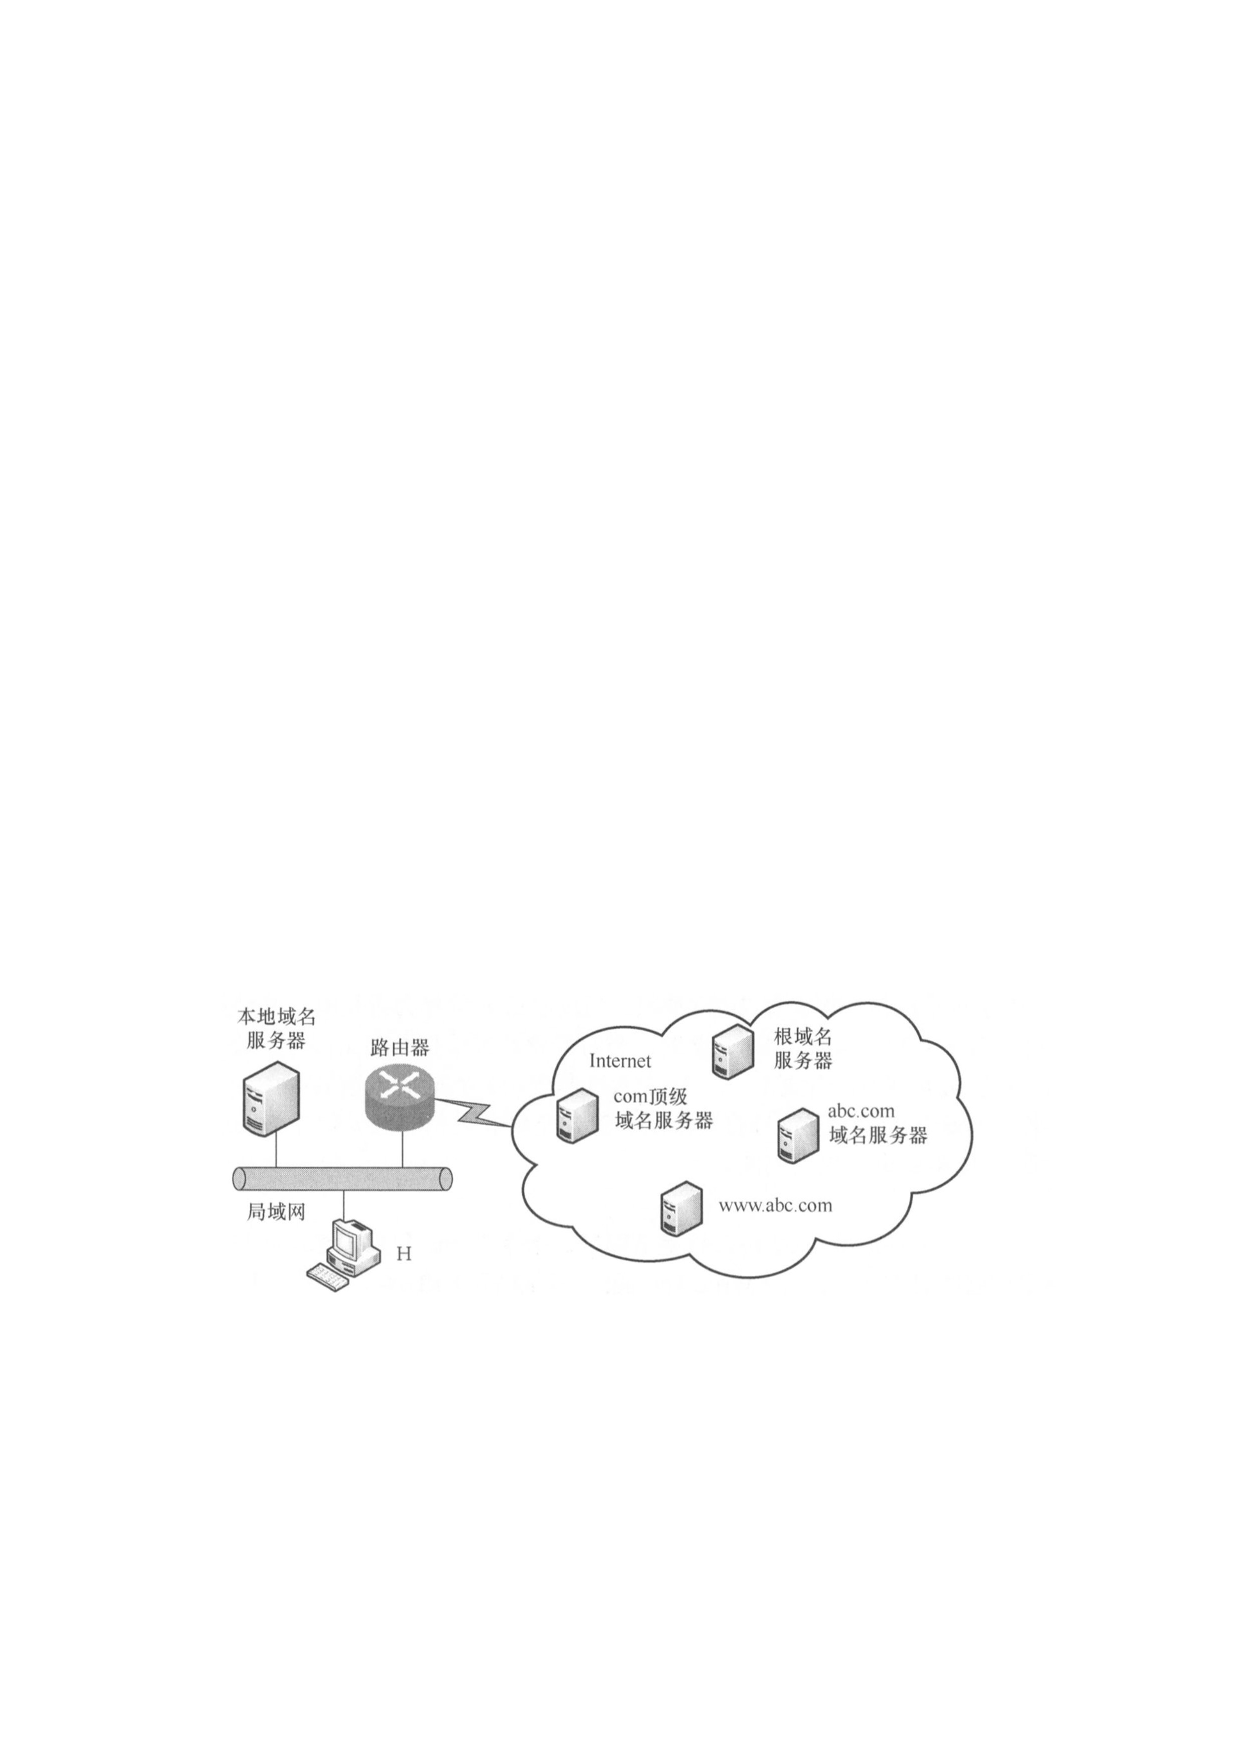
\includegraphics[width=.65\linewidth,height=.4\textheight,keepaspectratio]{../assets/figures/2020-questions-p005-b006.pdf}\end{center}

\begin{center}\begin{tabular}{>{\raggedright\arraybackslash}p{\dimexpr(\linewidth-8\tabcolsep)/4\relax}>{\raggedright\arraybackslash}p{\dimexpr(\linewidth-8\tabcolsep)/4\relax}>{\raggedright\arraybackslash}p{\dimexpr(\linewidth-8\tabcolsep)/4\relax}>{\raggedright\arraybackslash}p{\dimexpr(\linewidth-8\tabcolsep)/4\relax}}
\textbf{A.} 10ms, 40ms & \textbf{B.} 10ms, 50ms & \textbf{C.} 20ms, 40ms & \textbf{D.} 20ms, 50ms\\[.35em]\end{tabular}\end{center}

\subsection*{二、综合应用题（第41～47 小题，共70 分）}

41.（13 分）定义三元组\(\displaystyle (a,\allowbreak b,\allowbreak c)\)（其中a, b, c 均为正数）的距离。\(\displaystyle D=|a-b|+|b-c|\)。给定3 个非空整数集合\(\displaystyle S_1\)、\(\displaystyle S_2\)和\(\displaystyle S_3\)，按升序分别存储在3 个数组中。设计一个尽可能高效的算法，计算并输出所有可能的三元组\(\displaystyle (a,\allowbreak b,\allowbreak c)\)\(\displaystyle (a\in S_1,\allowbreak b\in S_2,\allowbreak c\in S_3)\)中的最小距离。例如\(\displaystyle S_1=\{-1,\allowbreak 0,\allowbreak 9\}\)，\(\displaystyle S_2=\{-25,\allowbreak -10,\allowbreak 10,\allowbreak 11\}\)，\(\displaystyle S_3=\{2,\allowbreak 9,\allowbreak 17,\allowbreak 30,\allowbreak 41\}\)，则最小距离为2，相应的三元组为(9, 10, 9)。要求： （1）给出算法的基本设计思想。 （2）根据设计思想，采用C 或C++语言描述算法，关键之处给出注释。 （3）说明你所设计算法的时间复杂度。


42.（10 分）若任一个字符的编码都不是其他字符编码的前缀，则称这种编码具有前缀特性。现有某字符集（字符个数≥2）的不等长编码，每个字符的编码均为二进制的0、1 序列，最长为 \(\displaystyle L\) 位，且具有前缀特性。请回答下列问题： （1）哪种数据结构适宜保存上述具有前缀特性的不等长编码？ （2）基于你所设计的数据结构，简述从0/1 串到字符串的译码过程。 （3）简述判定某字符集的不等长编码是否具有前缀特性的过程。


43.（13 分）有实现\(\displaystyle x\times y\) 的两个C 语言函数如下：


\begin{Verbatim}[breaklines,breakanywhere,fontsize=\small]
unsigned umul (unsigned x, unsigned y) { return x*y; }
int imul (int x, int y) { return x * y; }
\end{Verbatim}

假定某计算机M 中ALU 只能进行加法计算和逻辑运算。请回答下列问题。 （1）若M 的指令系统中没有乘法指令，但有加法、减法和位移等指令，则在M 上也能实现上述两个函数中的乘法运算，为什么？ （2）若M 的指令系统中有乘法指令，则基于ALU、位移器、寄存器以及相应控制逻辑实现乘法指令时，控制逻辑的作用是什么？ （3）针对以下三种情况：\textcircled{1}没有乘法指令；\textcircled{2}有使用ALU 和位移器实现的乘法指令；\textcircled{3}有使用阵列乘法器实现的乘法指令，函数umul()在哪种情况下执行时间最长？哪种情况下执行的时间最短？说明理由 （4）n 位整数乘法指令可保存\(\displaystyle 2n\) 位乘积，当仅取低n 位作为乘积时，其结果可能会发生溢出。 当\(\displaystyle n=32,\allowbreak \ x=2^{31}-1,\allowbreak \ y=2\) 时，带符号整数乘法指令和无符号整数乘法指令得到的\(\displaystyle x\times y\) 的\(\displaystyle 2n\) 位乘积分别是什么（用十六进制表示）？此时函数umul()和imul()的返回结果是否溢出？对于无符号整数乘法运算，当仅取乘积的低n 位作为乘法结果时，如何用\(\displaystyle 2n\) 位乘积进行溢出判断？


44.（10 分）假定主存地址为32 位，按字节编址，指令Cache 和数据Cache 与主存之间均采用8 路组相联映射方式，直写（Write Through）写策略和LRU 替换算法，主存块大小为64B，数据区容量各为32KB。开始时Cache 均为空。请回答下列问题。 （1）Cache 每一行中标记（Tag）、LRU 位各占几位？是否有修改位？ （2）有如下C 语言程序段：


\begin{Verbatim}[breaklines,breakanywhere,fontsize=\small]
for (k = 0; k < 1024 ; k++)
    s[k] = 2 * s[k];
\end{Verbatim}

若数组s 及其变量k 均为int 型，int 型数据占4B,变量k 分配在寄存器中，数组s 在主存中的起始地址为0080 00C0H，则该程序段执行过程中，访问数组s 的数据Cache 缺失次数为多少？ （3）若CPU 最先开始的访问操作是读取主存单元0001 0003H 中的指令，简要说明从Cache 中访问该指令的过程，包括Cache 缺失处理过程。


45.（7 分）现有5 个操作A、B、C、D 和E，操作C 必须在A 和B 完成后执行，操作E 必须在C 和D 完成后执行，请使用信号量的wait()、signal()操作（P、V 操作）描述上述操作之间的同步关系，并说明所用信号量及其初值。


46.（8 分）某32 位系统采用基于二级页表的请求分页存储管理方式，按字节编址，页目录项和页表项长度均为4 字节，虚拟地址结构如下所示。 


\begin{center}\begin{adjustbox}{max width=\linewidth}\begin{tabular}{|>{\raggedright\arraybackslash}p{\dimexpr(\linewidth-6\tabcolsep-4\arrayrulewidth)/3\relax}|>{\raggedright\arraybackslash}p{\dimexpr(\linewidth-6\tabcolsep-4\arrayrulewidth)/3\relax}|>{\raggedright\arraybackslash}p{\dimexpr(\linewidth-6\tabcolsep-4\arrayrulewidth)/3\relax}|}\hline
页目录号（10位） & 页号（10位） & 页内偏移量（12位）\\\hline\end{tabular}\end{adjustbox}\end{center}

某C 程序中数组a[1024][1024]的起始虚拟地址为1080 0000H，数组元素占4 字节，该程序运行时，其进程的页目录起始物理地址为0020 1000H，请回答下列问题。 （1）数组元素a[1][2]的虚拟地址是什么？对应的页目录号和页号分别是什么？对应的页目录项的物理地址是什么？若该目录项中存放的页框号为00301H，则a[1][2]所在页对应的页表项的物理地址是什么？ （2）数组a 在虚拟地址空间中所占的区域是否必须连续？在物理地址空间中所占区域是否必须连续？ （3）已知数组a 按行优先方式存放，若对数组a 分别按行遍历和按列遍历，则哪种遍历方式的局部性更好？


47.（9 分）某校园网有两个局域网，通过路由器R1、R2 和R3 互联后接入Internet，S1 和S2 为以太网交换机。局域网采用静态IP 地址配置，路由器部分接口以及各主机的IP 地址如下图所示。 


\begin{center}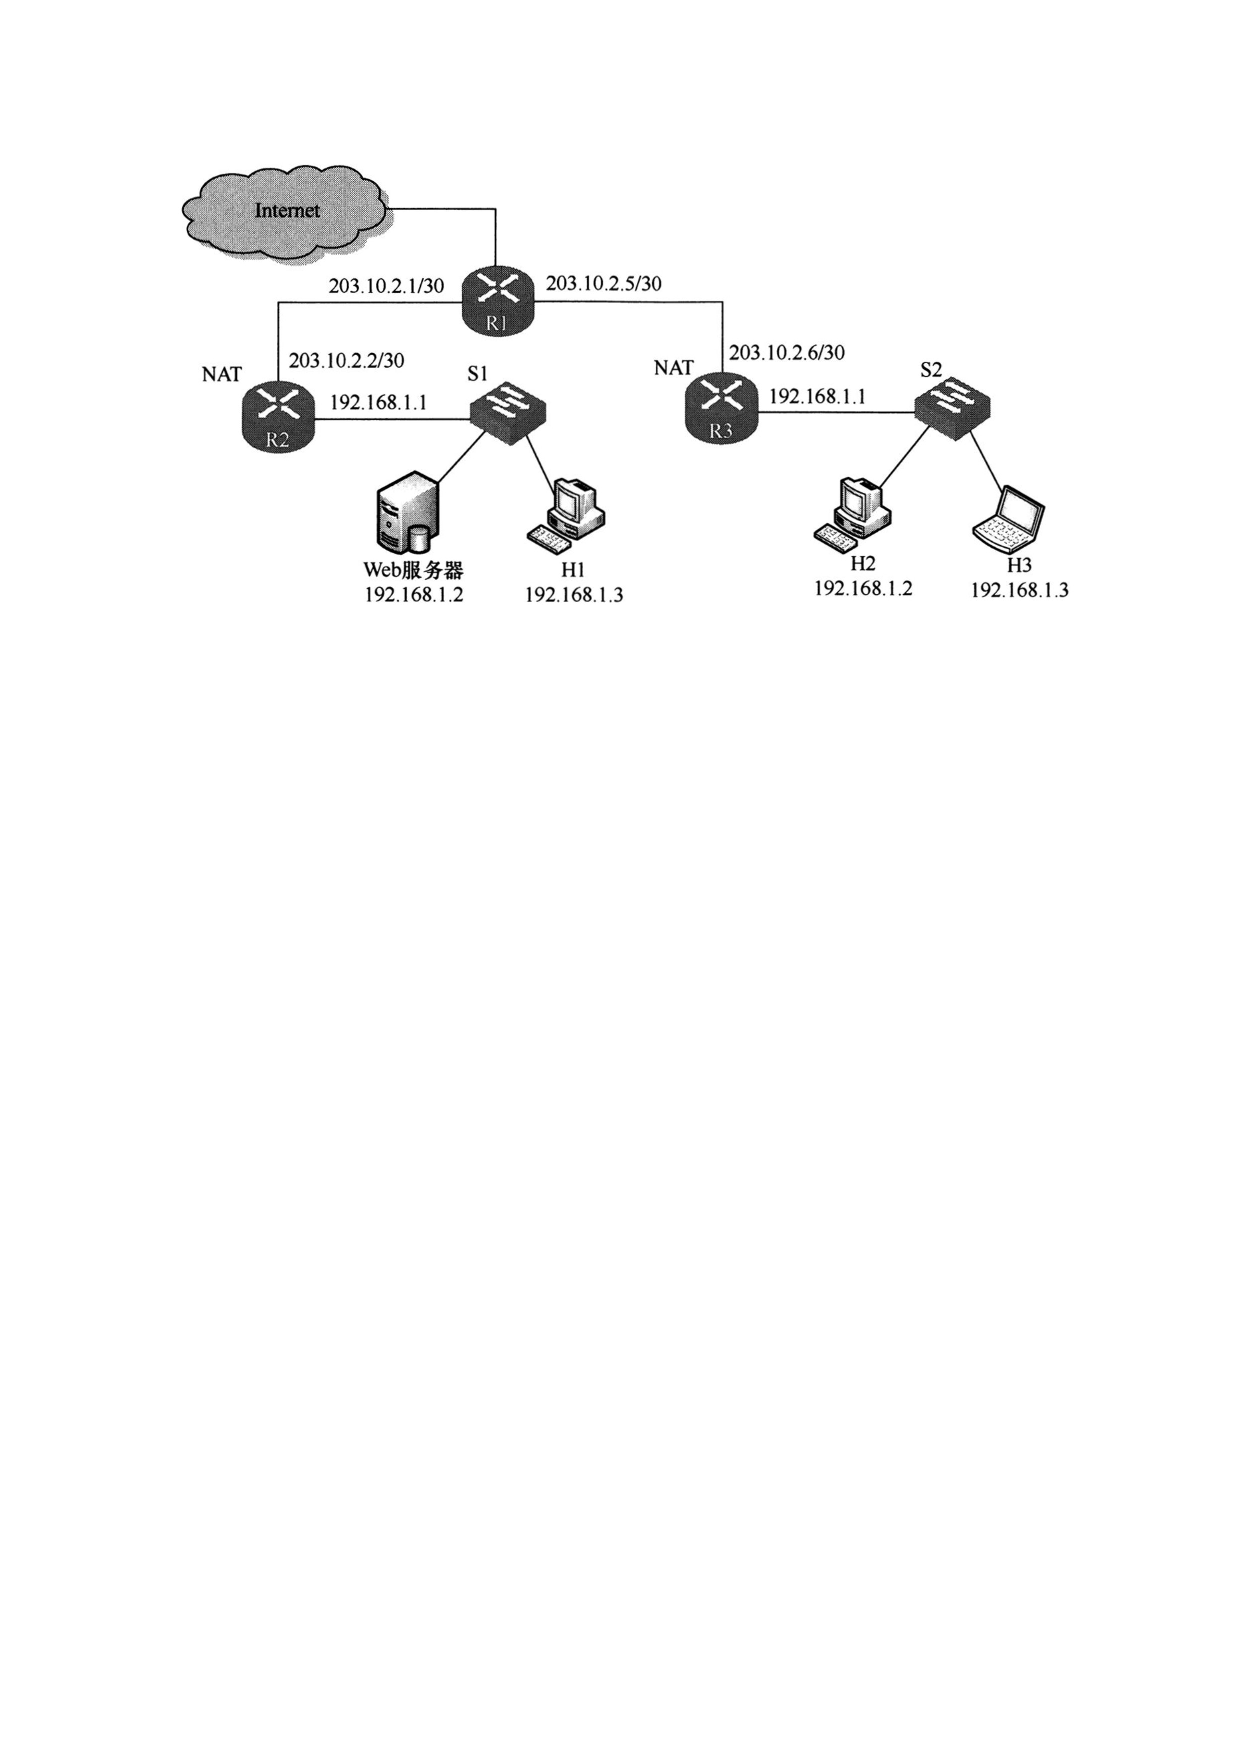
\includegraphics[width=.65\linewidth,height=.4\textheight,keepaspectratio]{../assets/figures/2020-questions-p012-b001.pdf}\end{center}

假设NAT转换表结构为：


\begin{center}\begin{adjustbox}{max width=\linewidth}\begin{tabular}{|>{\raggedright\arraybackslash}p{\dimexpr(\linewidth-8\tabcolsep-5\arrayrulewidth)/4\relax}|>{\raggedright\arraybackslash}p{\dimexpr(\linewidth-8\tabcolsep-5\arrayrulewidth)/4\relax}|>{\raggedright\arraybackslash}p{\dimexpr(\linewidth-8\tabcolsep-5\arrayrulewidth)/4\relax}|>{\raggedright\arraybackslash}p{\dimexpr(\linewidth-8\tabcolsep-5\arrayrulewidth)/4\relax}|}\hline
外网 IP地址 & 外网 端口号 & 内网 IP地址 & 内网 端口号\\\hline
 &  &  & \\\hline\end{tabular}\end{adjustbox}\end{center}

请回答下列问题： （1）为使H2 和H3 能够访问Web 服务器（使用默认端口号），需要进行什么配置？ （2）若H2 主动访问Web 服务器时，将HTTP 请求报文封装到IP 数据报P 中发送，则H2 发送 P 的源IP 地址和目的IP 地址分别是什么？经过R3 转发后，P 的源IP 地址和目的IP 地址分别是什么？经过R2 转发后，P 的源IP 地址和目的IP 地址分别是什么？

\end{document}
